\scanpage{24}
\margin{Mireille \& enfants}
\figure{
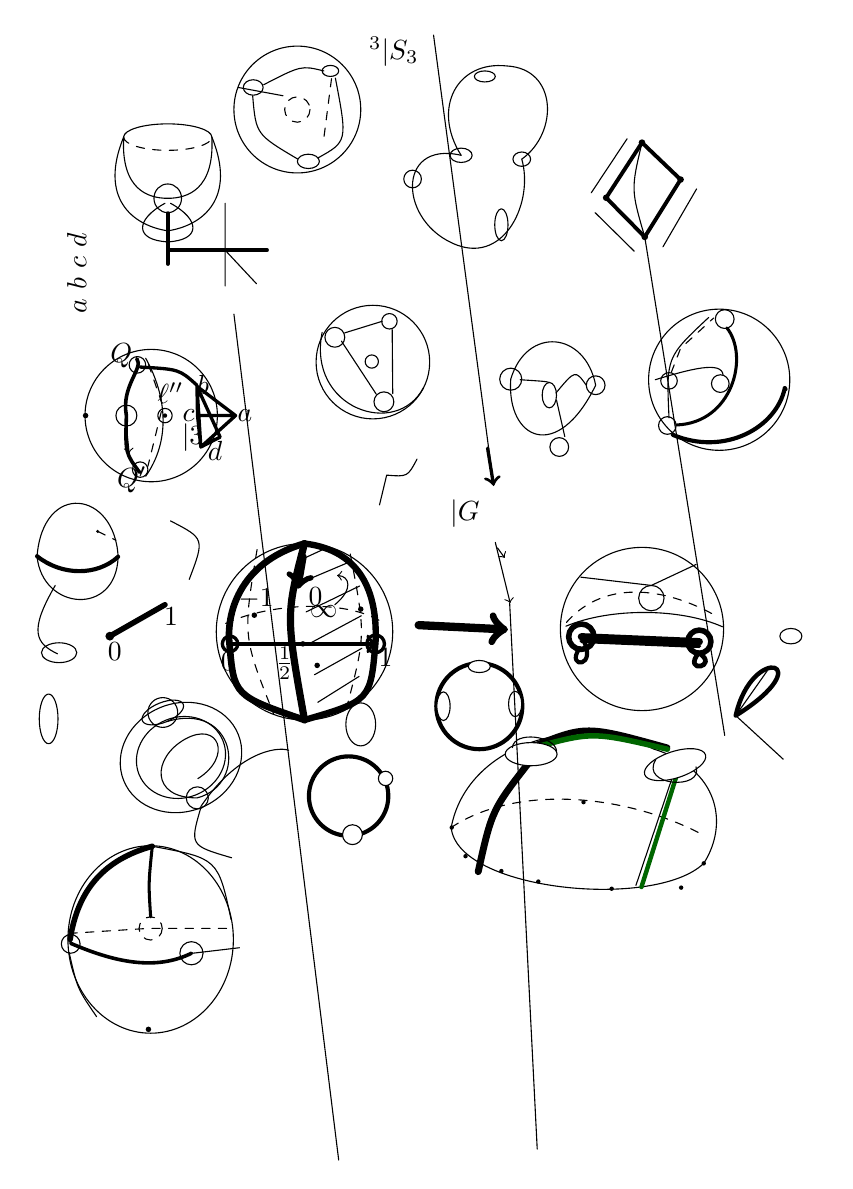
\begin{tikzpicture}[x=.007cm,y=-.007cm,line cap=round,line join=round]
\begin{scope}[shift={(330,425)}]
\draw (-80,-80) arc[start angle=180,end angle=360,x radius=80,y radius=24];
\draw[dashed] (-80,-80) arc[start angle=180,end angle=0,x radius=80,y radius=24];
\draw (-80,-80) .. controls (-125,30) and (-65,80) .. (0,90) .. controls (65,80) and (125,30) .. (80,-80);
\draw (-80,-80) .. controls (-85,15) and (-36,31) .. (0,31) .. controls (36,31) and (85,15) .. (80,-80);
\draw (0,31) ellipse (25 and 26);
\draw (-5,40) .. controls (-60,70) and (-60,107) .. (0,110) .. controls (60,107) and (60,70) .. (5,40);
\draw[line width=1.4pt] (0,58)--(0,125)--(180,125) (0,98)--(0,150);
\draw (104,40)--(104,190) (104,125)--(161,186);
\end{scope}
\begin{scope}[shift={(565,295)}]
\draw (0,0) circle (115);
\draw (-80,-40) ellipse (18 and 14) (20,94) ellipse (20 and 13) (60,-70) ellipse (15 and 10);
\draw (-81,-25) .. controls (-75,45) .. (1,90) (37,88) .. controls (91,58) .. (69,-57);
\draw (-61,-45) .. controls (7,-80) .. (48,-70);
\draw[dashed] (62,-56)--(47,60) (0,0) circle (23);
\draw (-107,-40)--(-26,-25);
\end{scope}
\node at (740,190) {\(\unsure{\circlearrowleft^{3}|\mathfrak S_3}\)};
\begin{scope}[shift={(900,380)}]
\draw (-38,-2) .. controls (-92,-88) and (-45,-174) .. (45,-164) .. controls (137,-159) and (139,-43) .. (72,5);
\draw (-38,-2) ellipse (20 and 13) (72,5) ellipse (16 and 13) (5,-145) ellipse (19 and 10);
\draw (-38,-2) .. controls (-157,-30) and (-152,121) .. (-45,161) .. controls (42,193) and (94,82) .. (72,5);
\draw (-126,41) circle (16);
\draw (35,124) ellipse (12 and 29);
\end{scope}
\draw (812,160)--(921,977);
\draw[->,line width=1.2pt] (910,909)--(921,977);
\node at (869,1028) {\(\unsure{\circlearrowleft|G}\)};
\draw[->] (924,1080)--(951,1190);
\draw[->] (928,1090)--(941,1108);
\draw (450,666)--(640,2200);
\draw (714,1012)--(727,958) .. controls (765,961) .. (782,929);
\draw (335,1041) .. controls (397,1073) .. (369,1147);
\begin{scope}[shift={(1190,440)}]
\draw[line width=1.4pt] (0,-85)--(-65,15)--(5,86)--(70,-18)--cycle;
\draw (0,-85) .. controls (-20,0) .. (5,86);
\foreach \x/\y in {0/-85,-65/15,5/86,70/-18}{\fill (\x,\y) circle (6);}
\draw (-92,6)--(-27,-92) (-85,42)--(-14,112) (38,104)--(99,-1);
\end{scope}
\draw (1195,526)--(1340,1430);
\begin{scope}[shift={(300,850)},rotate=-90]
\draw (0,0) circle (120);
\draw[line width=1.3pt] (-103,26) .. controls (-86,13) and (-54,55) .. (0,45) .. controls (68,47) .. (103,21);
\draw (-104,10) .. controls (-34,-29) and (46,-35) .. (110,10);
\draw[dashed] (-93,5)--(-18,-21)--(92,6);
\draw (-92,25) circle (15) (98,20) circle (14) (0,-25) circle (13);
\draw (0,45) circle (19);
\fill (0,-25) circle (4);
\fill (0,119) circle (5);
\draw[line width=1.2pt] (-88,20) .. controls (-84,-51) .. (-55,-83);
\draw[line width=1.2pt] (-53,-83)--(0,-153)--(57,-90)--(-53,-83)--(0,-84)--(0,-153) (-53,-83)--(39,-125)--(57,-90) (0,-84)--(57,-90);
\node at (0,-170) {\(a\)};
\node at (-55,-94) {\(\unsure{b}\)};
\node at (0,-68) {\(\unsure{c}\)};
\node at (64,-116) {\(\unsure{d}\)};
\node at (40,-75) {\(\unsure{\circlearrowleft|3}\)};
\node at (-40,-35) {\(\ell''\)};
\node at (-108,54) {\(Q\)};
\node at (117,35) {\(Q'\)};
\draw[->] (18,45)--(68,40);
\end{scope}
\node[rotate=90] at (165,592) {\(a\ b\ c\ d\)};
\begin{scope}[shift={(702,753)}]
\draw (0,0) circle (103);
\draw (-69,-45) circle (18) (30,-74) circle (14) (20,72) circle (18) (-2,-1) circle (12);
\draw (-57,-38)--(6,58) (36,57)--(35,-60) (17,-74)--(-51,-53);
\draw (-92,-54) .. controls (-120,84) and (43,140) .. (92,46);
\end{scope}
\begin{scope}[shift={(1030,802)}]
\draw (-78,-18) .. controls (-86,91) and (6,136) .. (76,-7) .. controls (57,-105) and (-49,-115) .. (-78,-18);
\draw (-78,-18) circle (20) (76,-7) circle (17) (10,105) circle (17);
\draw (-8,11) ellipse (13 and 23);
\draw (-61,-17) .. controls (-15,-14) .. (-8,-12) (5,20)--(20,86) (4,7) .. controls (39,-35) .. (59,-7);
\end{scope}
\begin{scope}[shift={(1330,785)}]
\draw (0,0) circle (128);
\draw (-94,83) circle (16) (2,7) circle (16) (10,-110) circle (17) (-91,2) circle (15);
\draw[line width=1.1pt] (-77,82) .. controls (24,78) and (55,-42) .. (14,-94);
\draw[line width=1.5pt] (-84,100) .. controls (10,139) and (104,87) .. (119,15);
\draw (-91,69) .. controls (-96,-41) .. (-19,-113);
\draw[dashed] (-87,-13)--(-70,-57)--(-10,-112);
\draw (-116,0) .. controls (-50,-20) and (4,-34) .. (7,-9);
\fill (120,17) circle (4);
\end{scope}
\begin{scope}[shift={(168,1110)}]
\draw (-75,-5) .. controls (-64,-142) and (66,-124) .. (72,-4) .. controls (69,105) and (-66,94) .. (-75,-5);
\draw[line width=1.5pt] (-75,-5) .. controls (-30,31) and (34,31) .. (72,-4);
\fill (35,-50) circle (3);
\draw[dashed] (35,-50)--(68,-34);
\draw (-42,48) .. controls (-91,132) and (-77,153) .. (-38,172);
\draw (-35,170) ellipse (32 and 18);
\end{scope}
\draw[line width=2pt] (225,1250)--(325,1193);
\fill (225,1250) circle (8);
\node at (234,1278) {\(0\)};
\node at (336,1214) {\(1\)};
\draw (114,1400) ellipse (17 and 45);
\begin{scope}[shift={(578,1242)}]
\draw (0,0) circle (160);
\draw[line width=2.4pt] (0,-160) .. controls (-121,-125) and (-142,-29) .. (-136,22) .. controls (-128,116) .. (0,160);
\draw[line width=2.3pt] (0,-160) .. controls (102,-148) and (132,-71) .. (129,16) .. controls (120,125) .. (0,160);
\draw[line width=2.6pt] (0,-160) .. controls (-34,-30) .. (0,160);
\draw[->,line width=2.4pt] (-2,-136)--(-12,-78);
\draw[->,line width=1.4pt] (-138,22)--(131,22);
\draw[dashed] (-143,-15) .. controls (-71,-49) and (72,-63) .. (143,-16);
\draw[dashed] (-86,-149) .. controls (-112,8) .. (-56,149) (83,-141) .. controls (111,6) .. (76,139);
\foreach \x/\y in {-135/22,-3/22,129/22,-91/-30,102/-41,23/61,0/156}{\fill (\x,\y) circle (5);}
\draw[line width=1.2pt] (-135,22) circle (14) (129,22) circle (16);
\foreach \a/\b/\c/\d in {3/-135/42/-153,0/-92/78/-125,3/-36/100/-83,8/22/103/-29,18/78/104/30,24/128/99/81}{\draw (\a,\b)--(\c,\d);}
\draw[->] (55,-49) .. controls (89,-77) and (82,-101) .. (59,-102);
\node at (-88,-60) {\(-1\)};
\node at (-36,57) {\(\frac12\)};
\node at (20,-64) {\(\unsure{0}\)};
\node at (35,-37) {\(\unsure{\infty}\)};
\node at (-139,55) {\(\unsure{0}\)};
\node at (147,46) {\(\unsure{1}\)};
\end{scope}
\draw[->,line width=3pt] (785,1230)--(947,1238);
\begin{scope}[shift={(1190,1237)}]
\draw (0,0) circle (148);
\draw (-138,-5) .. controls (-57,-39) and (70,-38) .. (146,-4);
\draw[dashed] (-137,-12) .. controls (-64,-95) and (52,-72) .. (139,-21);
\draw[line width=1.4pt] (-110,22)--(104,31);
\draw[line width=2.6pt] (-110,14)--(104,23);
\draw[line width=2pt] (-110,14) circle (23) (104,23) circle (21);
\draw (17,-56) circle (23);
\draw (-111,-94)--(17,-79)--(98,-117);
\draw[line width=1.5pt] (-113,35) .. controls (-141,73) and (-75,72) .. (-110,14);
\draw[line width=1.7pt] (103,43) .. controls (72,82) and (142,69) .. (103,43);
\end{scope}
\draw (1460,1250) ellipse (20 and 14);
\draw[line width=1.6pt] (1360,1394) .. controls (1390,1261) and (1517,1296) .. (1360,1394);
\draw (1360,1394)--(1446,1473) (1360,1394)--(1417,1313);
\draw (680,1410) ellipse (27 and 39);
\begin{scope}[shift={(895,1377)}]
\draw[line width=1.5pt] (0,0) circle (78);
\draw[fill=white] (-65,0) ellipse (12 and 26) (65,-4) ellipse (12 and 23) (0,-72) ellipse (20 and 11);
\end{scope}
\begin{scope}[shift={(354,1470)},rotate=22]
\draw (0,0) ellipse (112 and 98);
\draw (0,0) ellipse (82 and 73);
\draw (0,-88) ellipse (40 and 18);
\draw (0,-88) circle (27);
\draw (0,79) circle (20);
\draw (0,-70) .. controls (130,-59) and (97,91) .. (0,79) .. controls (-79,48) and (-49,-19) .. (19,-28) .. controls (89,-37) and (88,34) .. (14,47);
\draw (0,97) .. controls (-45,154) .. (17,203);
\draw (0,96) .. controls (96,31) and (167,45) .. (186,61);
\end{scope}
\begin{scope}[shift={(658,1540)}]
\draw[line width=1.5pt] (0,0) circle (72);
\draw[fill=white] (7,70) circle (18) (67,-32) circle (13);
\draw[dashed] (-66,-32)--(-44,-59);
\end{scope}
\begin{scope}[shift={(299,1800)}]
\draw (0,0) ellipse (150 and 170);
\draw[line width=2pt] (-146,0) .. controls (-130,-105) and (-69,-149) .. (3,-169);
\draw (3,-169) .. controls (122,-147) .. (146,-36);
\draw[line width=1.3pt] (-145,7) .. controls (-68,40) and (7,58) .. (74,25);
\draw (76,25)--(161,15);
\draw[dashed] (-148,-11)--(-5,-20)--(139,-20);
\draw (-145,8) circle (17) (74,25) circle (21);
\draw[dashed] (0,-20) circle (21);
\draw[line width=1.1pt] (3,-169) .. controls (-4,-102) .. (0,-41);
\draw (-148,23) .. controls (-133,89) .. (-98,140);
\fill (-4,163) circle (5);
\end{scope}
\begin{scope}[shift={(1080,1557)}]
\draw (-236,40) .. controls (-208,-108) and (-15,-171) .. (132,-102) .. controls (249,-66) and (268,33) .. (222,105);
\draw (-236,40) .. controls (-225,155) and (134,190) .. (222,105);
\draw[dashed] (-236,40) .. controls (-115,-40) and (83,-20) .. (222,54);
\draw[line width=2.5pt] (-187,120) .. controls (-162,8) .. (-91,-83);
\draw[line width=2.2pt] (-91,-106) .. controls (8,-146) .. (156,-105);
\draw[green!40!black,line width=2pt] (-89,-104) .. controls (20,-134) .. (156,-102);
\draw[green!40!black,line width=1.6pt] (174,-58)--(109,148);
\draw (164,-48)--(99,145);
\draw[fill=white] (-91,-93) ellipse (47 and 21);
\draw (-125,-105) .. controls (-122,-136) and (-47,-126) .. (-45,-99);
\draw[fill=white,rotate around={18:(170,-74)}] (170,-74) ellipse (58 and 24);
\draw (135,-83) .. controls (105,-35) and (222,-27) .. (208,-70);
\foreach \x/\y in {-235/40,-210/92,-145/119,-78/138,55/151,181/149,222/105,4/-6}{\fill (\x,\y) circle (4);}
\end{scope}
\draw (950,1190)--(1000,2180);
\end{tikzpicture}
}% crop-candidate: scan 24
\margin{\(\operatorname{diag}_Q\simeq\omega_Q\)\quad
\(\operatorname{diag}_Q\wedge\omega_Q\simeq\operatorname{codiag}_Q\)}
\margin{\unsure{avec} un ens à trois éléments, on fait \(3\times2=6\) courbes \unsure{elliptiques} de type \((1,1)\)}
avec un ens \(I\) de card \(4\),
\unsure{on} trouve \(\unsure{17|14}\) \unsure{points|ponts} \unsure{or|ou} canoniques \inserted{de type \((0,4)\)}
\((14=3\times4+\deleted{3\times}2)\)
dont deux tétraèdres,
\deleted{quatre}\inserted{trois} carrés, \deleted{deux} \(2\times3=6\)
assemblages de \deleted{\unsure{F}} ``T'' droits,
\(6=2\times3\) assemblages de \inserted{\(1\)} T gauches.
\margin{23}
